\documentclass[hyperref={pdfpagelabels=false}]{beamer}
\usepackage{lmodern}
\usepackage{graphicx}

\usetheme{Goettingen}
\title{An Radial Basis Network to Describe The Antibody Antigen Interactions}  
\author{Liu Chuanxing} 
\date{\today} 
\begin{document}
\logo{\includegraphics[scale=0.14]{logo-SF}}
\begin{frame}
\titlepage
\end{frame} 


\begin{frame}
\frametitle{Table of contents}
\tableofcontents
\end{frame} 


\section{Introduction} 
\subsection{Significance}
\begin{frame}
\frametitle{Significance} 
\begin{figure}
	\centering
	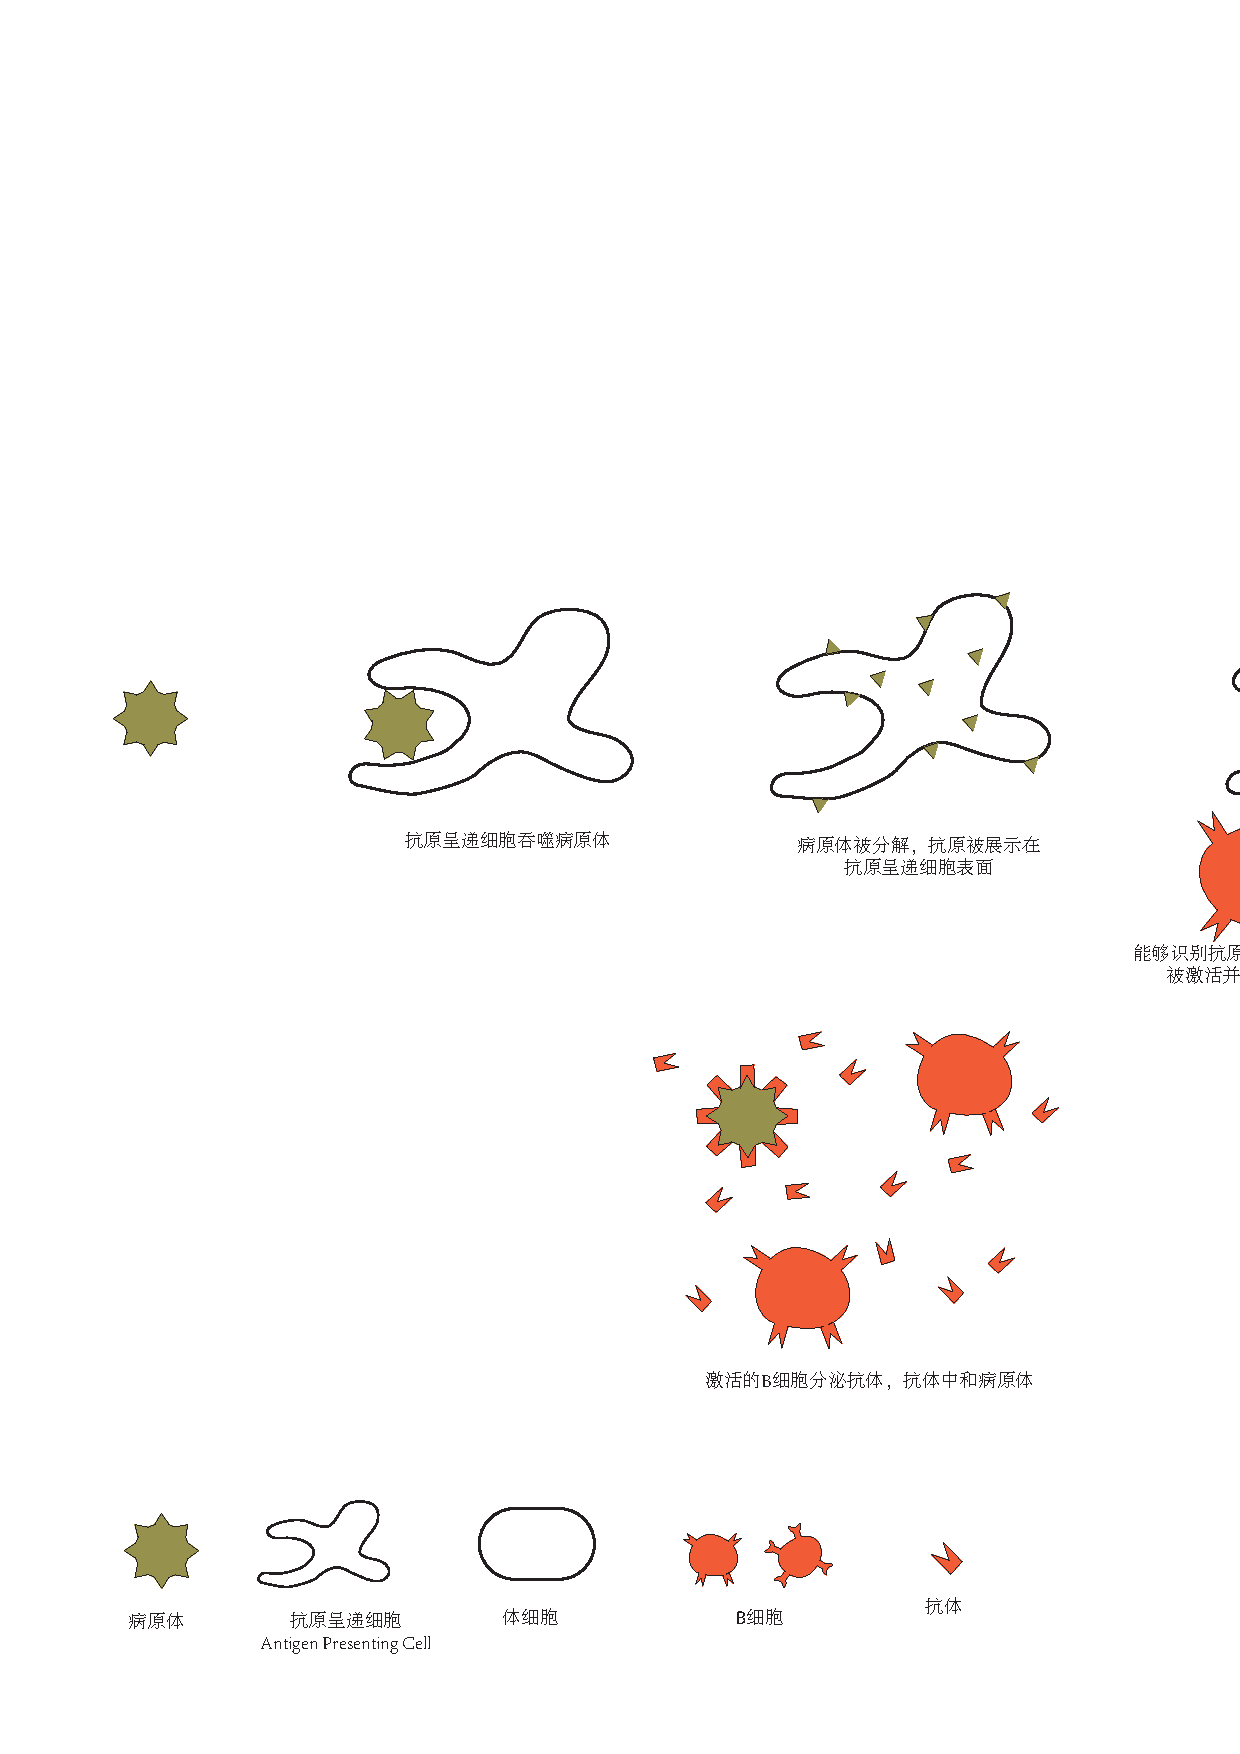
\includegraphics[scale=0.2]{SerumImmune}
	\caption{An illustration of serum immunity}
\end{figure}
\begin{itemize}
	\item Design therapeutic antibodies
	\item Design effective vaccines
\end{itemize}
\end{frame}

\subsection{The Problem}
\begin{frame}
\frametitle{The Problem} 
Do similar B-cell epitopes interact with similar paratopes?
\vspace{0.3cm}

Here is a similar research about TCR and its epitopes

\begin{figure}
	\centering
	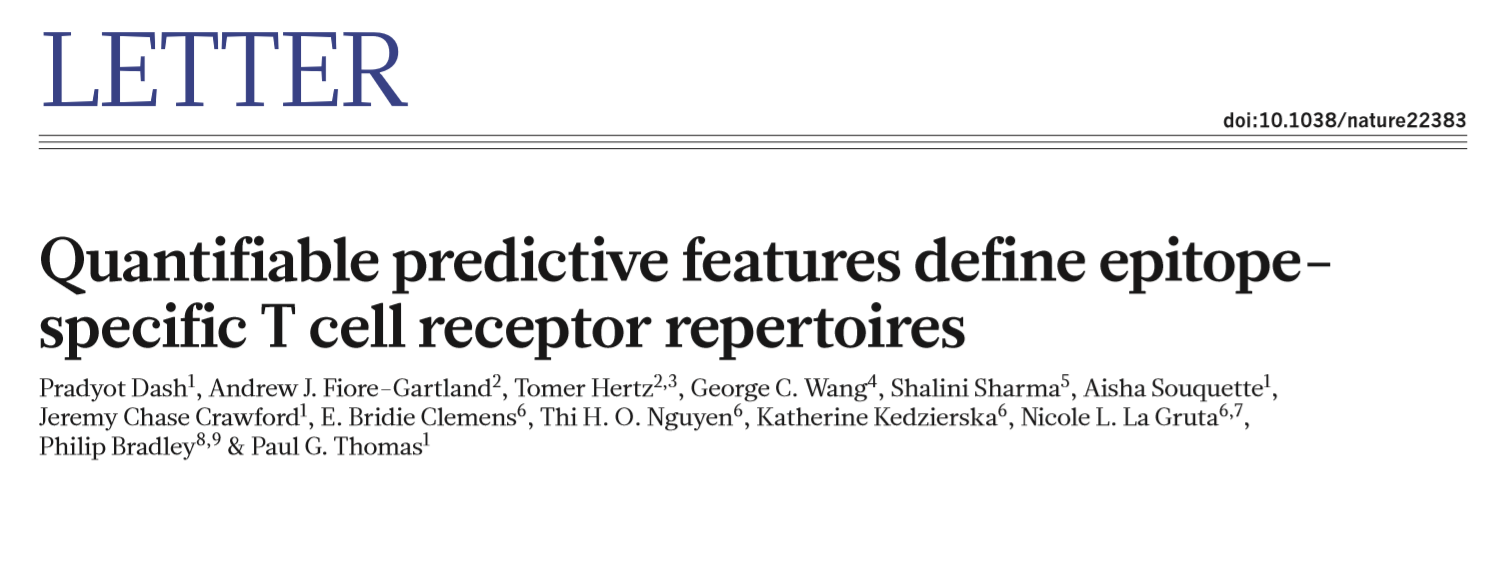
\includegraphics[scale=0.2]{Quantifiable_TCR}
\end{figure}

\begin{figure}
	\centering
	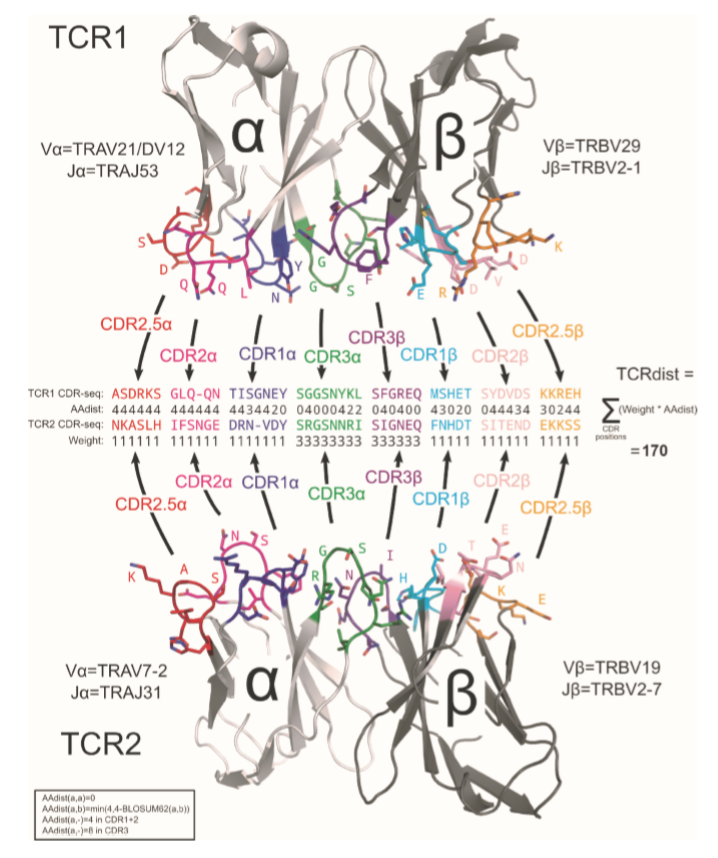
\includegraphics[scale=0.3]{figure9}
\end{figure}
\end{frame}

\subsection{The Challenge and the solution}
\begin{frame}
\frametitle{The Challenge} 
The interactions between B-cell epitopes and paratopes are conformational!

\begin{figure}
	\centering
	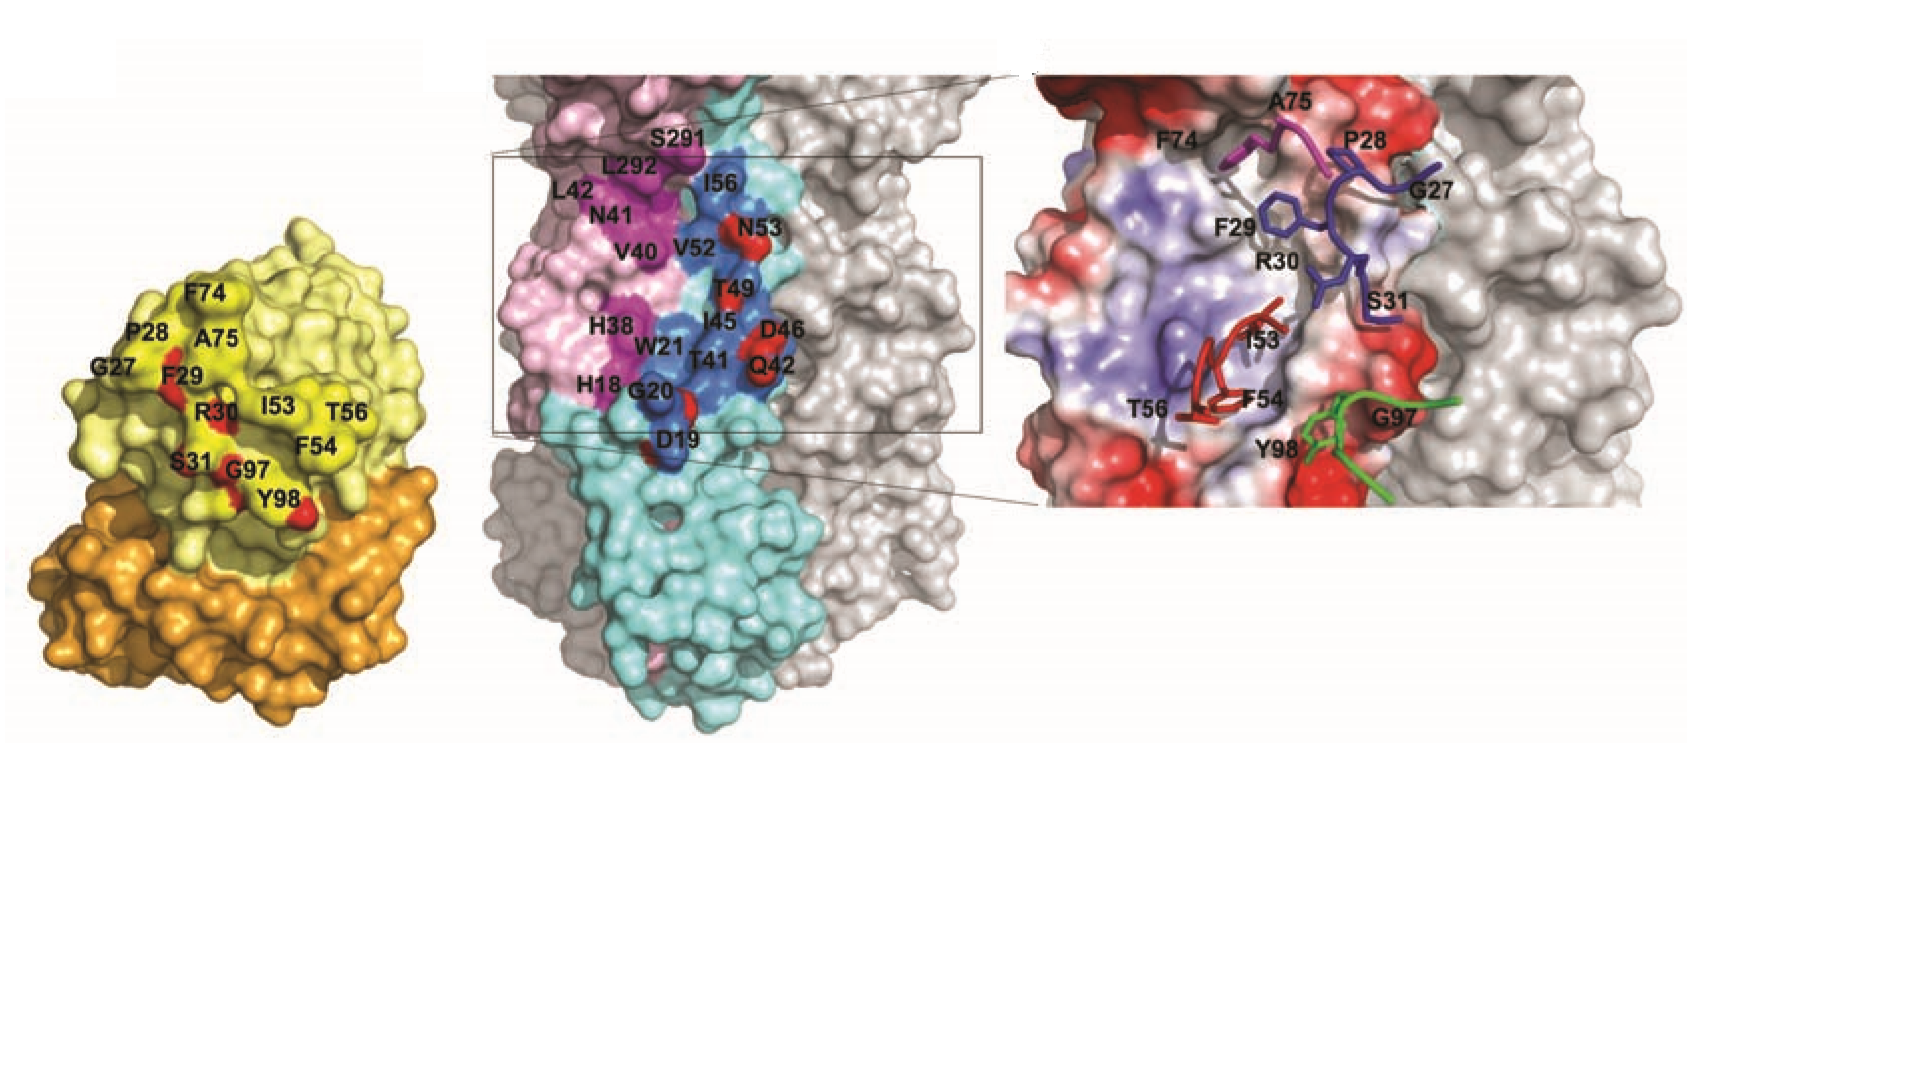
\includegraphics[scale=0.25]{ConformationalEpitope2}	
	\vspace{-2cm}
	\caption{\small{The interaction between Hemagglutinin and one of its antibodies}}
\end{figure}
\end{frame}

\begin{frame}
\frametitle{Solution of the challenge} 
We solved the challenge by focusing on the key amino acids(hot spots). As long as the sequence is short enough, the hot spots are composed of continuous sequences.
\vspace{0.3cm}

\begin{figure}[H]
	\centering
	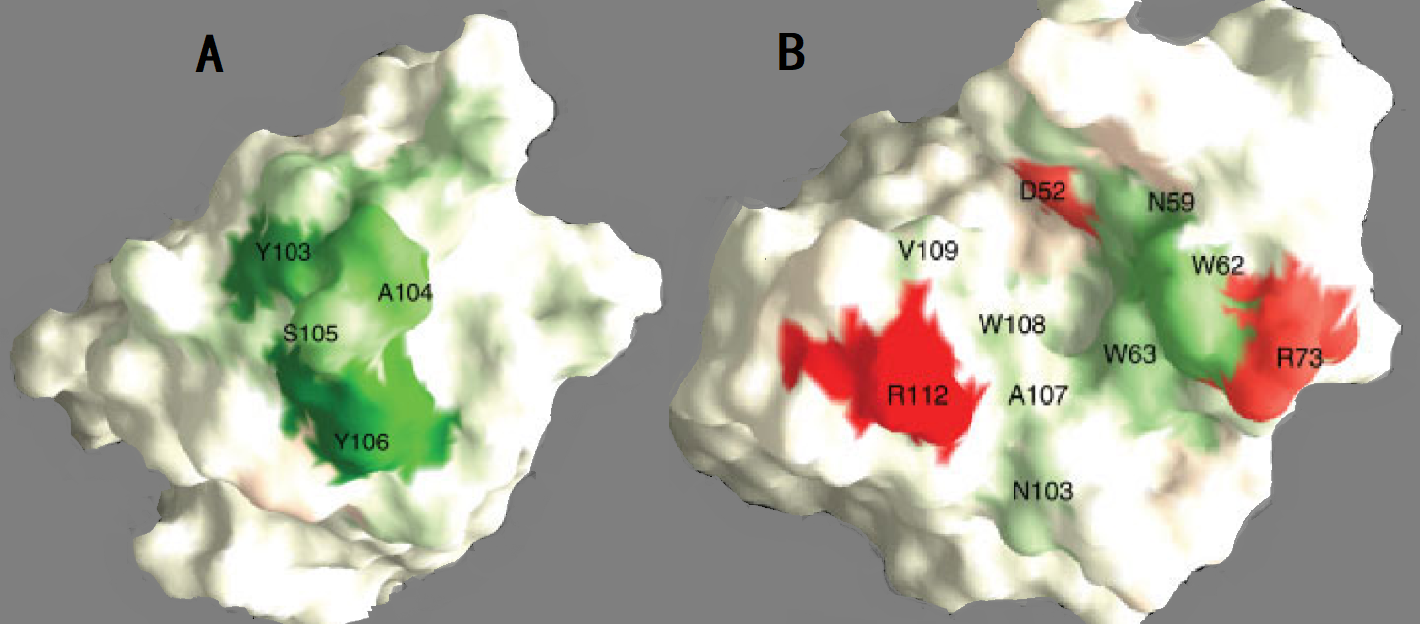
\includegraphics[scale=0.25]{HotSpot}	
%	\vspace{-2cm}
	\caption{\small{The hot spots between Hen Egg Lysozym(HEL) and one of its antibodies cAB-Lys3 }}
\end{figure}
\end{frame}
%\subsection{Subsection no.1.1  }
%\begin{frame}
%Without title somethink is missing. 
%\end{frame}
\subsection{The outline of our research}
\begin{frame}
\frametitle{The outline of our research}
	\begin{itemize}
		\item Data extraction
		\item Develop an Radial Basis Function Network(RBFN)
		\item Use the RBFN to tell the difference between the antibody amino acids and the antigen amino acids.
		\item Use the RBFN to predict how a mutation can affect the affinity of an antibody-antigen complex.
	\end{itemize}
\end{frame}

\section{Data Extraction} 
\subsection{Complexes, CDRs, Contact Number}
\begin{frame}
	\frametitle{Complex, CDR, Interacting Pairs}
	\begin{itemize}
		\item 1624 antibody-antigen complexes with resolution $\leq3A$.
		
		\item The CDRs are defined as follows
		\begin{table}[H]

\scalebox{0.8}{
\begin{tabular}{llll}
\hline\hline
 & CDR1      & CDR2     & CDR3 \\
\hline
Max-CDRL& 24 to 41       & 50 to 64        & 90 to 108       \\
\hline
Max-CDRH& 26 to 38       & 51 to 72        & 100 to 130       \\
\hline
\end{tabular}}
\caption{Locations of the CDRs}\label{CDRs_Range}
\end{table}
\item A and B are two amino acids, the contact number between A and B is defined as 
$$\text{CN}(A,B)=\sum\limits_{a\in A}\sum\limits_{b\in B} \chi\{d(a,b) \leq 4\}$$
\small{$a\in A $ means a is an atom in A and a is not a hydrogen atom. }
	\end{itemize}
\end{frame}

\subsection{Reduce Redundance}
\begin{frame}
	\frametitle{Define distance}
	\vspace{-1.5cm}
	The redundance reduction was based on the similarity of the CDRs. Each light/heavy chain was an individual.

		\begin{itemize}
			\item 	\textbf{Scoring rules}
	$$S(a,a)=1;\quad S(a,b) = 0; \quad S(a, -) = 0$$
			\item  \textbf{Calculate the distance}
		Concatenate the three CDRs. Suppose A and B are two concatenated CDRs of two light/heavy chains.
	$D(A, B) = 1- S(A, B)/N$
	where $N=min(Len(A), Len(B))$.
		\end{itemize}
\end{frame}
\begin{frame}
\frametitle{Select the cut-off distance}
\vspace{-1cm}
		\begin{figure}
			\includegraphics[scale=0.3]{ElbowMethod.eps}
		\end{figure}
\vspace{-1cm}
	According to the Elbow Method, we chose 0.1 as the cut-off distance.
\end{frame}

\begin{frame}
\frametitle{Select the representative from each cluster}
Suppose A is the set of all the amino acids for a given light/heavy chain, and $Ag$ is the set of all the amino acids in the corresponding antigen. The total contact number of A is defined as
$$TCN(A)=\sum\limits_{a\in A}\sum\limits_{b\in Ag}CN(a,b)$$

In each cluster, the chain with the largest TCN was selected as the representative.
\end{frame}

\subsection{Positive Cores, Negative Cores}
\begin{frame}
\frametitle{Positive cores and Negative cores}
\begin{itemize}
	\item \textbf{Match-type} was defined as the lengths of the interacting sequences. Match-type(2,3) means 2 consecutive antibody amino acids interacting with 3 consecutive antigen amino acids.

	\item For a light/heavy chain and a match-type(m,n), the core is defined as the interacting sequences of match-type(m,n), with the largest contact number.
	\item The negative cores were randomly generated sequences pairs which were not in the training set.
\end{itemize}
\end{frame}
	
\begin{frame}
\frametitle{What do we have?}
\begin{itemize}
		\item The training set of different match-types. For each match-type, the training set consists of the positive cores and the randomly generated negative cores. 
		\item The testing set of different match-types. For each match-type, there are 10 different testing sets, generated by combining the positive testing set with the 10 independently generated negative cores.
		\item The label for the positive cores is 1 and the label for the negative cores is -1.
	\end{itemize}
Here, the range of the match-type is $$\{(m,n): m,n = 1, 2, 3\}$$. 
\end{frame}
%\subsection{Lists I}
%\begin{frame}
%\frametitle{unnumbered lists}
%\begin{itemize}
%\item Introduction to  \LaTeX{}  
%\item Course 2 
%\item Termpapers and presentations with \LaTeX{}  
%\item Beamer class
%\end{itemize} 
%\end{frame}
%
%\begin{frame}\frametitle{lists with single pauses}
%\begin{itemize}
%\item Introduction to  \LaTeX{}  \pause 
%\item Course 2 \pause 
%\item Termpapers and presentations with \LaTeX{}  \pause 
%\item Beamer class
%\end{itemize} 
%\end{frame}
%
%\begin{frame}\frametitle{lists with pause}
%\begin{itemize}[<+->]
%\item Introduction to  \LaTeX{}  
%\item Course 2
%\item Termpapers and presentations with \LaTeX{}  
%\item Beamer class
%\end{itemize} 
%\end{frame}
%
%
%
%\subsection{Lists II}
%\begin{frame}\frametitle{numbered lists}
%\begin{enumerate}
%\item Introduction to  \LaTeX{}   
%\item Course 2 
%\item Termpapers and presentations with \LaTeX{}  
%\item Beamer class
%\end{enumerate}
%\end{frame}
%
%\begin{frame}
%\frametitle{numbered lists with single pauses}
%\begin{enumerate}
%\item Introduction to  \LaTeX{}  \pause 
%\item Course 2 \pause 
%\item Termpapers and presentations with \LaTeX{}  \pause 
%\item Beamer class
%\end{enumerate}
%\end{frame}
%
%\begin{frame}
%\frametitle{numbered lists with pause}
%\begin{enumerate}[<+->]
%\item Introduction to  \LaTeX{}  
%\item Course 2
%\item Termpapers and presentations with \LaTeX{}  
%\item Beamer class
%\end{enumerate}
%\end{frame}




\section{Develop an Radial Basis Function Network(RBFN)} 
\subsection{Define the distance between two cores}
\begin{frame}
\frametitle{The Substitution matrix}
\vspace{-1cm}
 		\begin{align*}
			\text{Substitution matrix} &= BLOSUM62\\
			\text{gap} &= Hp_1\\
			\text{extended gap} &= Hp_2\\
		\end{align*}
	Here $Hp_1$ and $Hp_2$ were two hyperparameters. We use the complete BLOSUM62, not the truncated BLOSUM62 as Pradyot Dash did. 
\end{frame}

\begin{frame}
\frametitle{The distance between two cores}
Suppose (Ab1, Ag1) and (Ab2, Ag2) are two cores of match-type(m,n). This distance between them is defined by the following steps.
	\begin{align*}
	S_{Ab} &= \mathrm{Aln}(\mathrm{Ab}_1, \mathrm{Ab}_2)\\
	S_{Ag} &= \mathrm{Aln}(\mathrm{Ag}_1, \mathrm{Ag}_2)\\
	S_{Ab}^{+} &= \frac{\mathrm{S_{Ab}} + 4\times m}{15 \times m}\\
	S_{Ag}^{+} &= \frac{\mathrm{S_{Ag}} + 4\times n}{15 \times n}\\
	S&=S_{Ab}^+ \times S_{Ag}^+\\
	D&= 1- S
	\end{align*}
$D$ is the distance defined.
\end{frame}

\subsection{Cross Validation and testing}
\begin{frame}
\frametitle{Cross Validation}
\begin{table}[H]\centering
\begin{tabular}{ccccc c}
\hline\hline
match-type   &  $Hp_1$     & $Hp_2$    & $r$   & $p$&average AUC\\
\hline
(1,1)  & -1  & -1 &0.0001&0.8&0.973\\
(1,2)  & -1  & -1 & 0.0001&0.8&0.860\\
(1,3)  & -1  & -1 &0.0001&0.8&0.834\\
(2,1)  & -1  & -1 &0.0001&0.8&0.870\\
(2,2)  & -1  & -1 &0.0001&0.8&0.842\\
(2,3)  & -1  & -1 &0.001&0.8&0.836\\
(3,1)  & -1  & -1 &0.0001&0.8&0.867\\
(3,2)  & -1  & -1 &0.001&0.8&0.862\\
(3,3)  & -1  & -1 &0.001&0.8&0.862\\
\hline
\end{tabular}
\caption{\small{We did a 5 cross validation. The best parameter are the values corresponding to the highest average AUC.}}
\label{Best_para_Binary}
\end{table}
\end{frame}


\begin{frame}
\frametitle{Testing the model}
\begin{figure}[H]
	\centering
	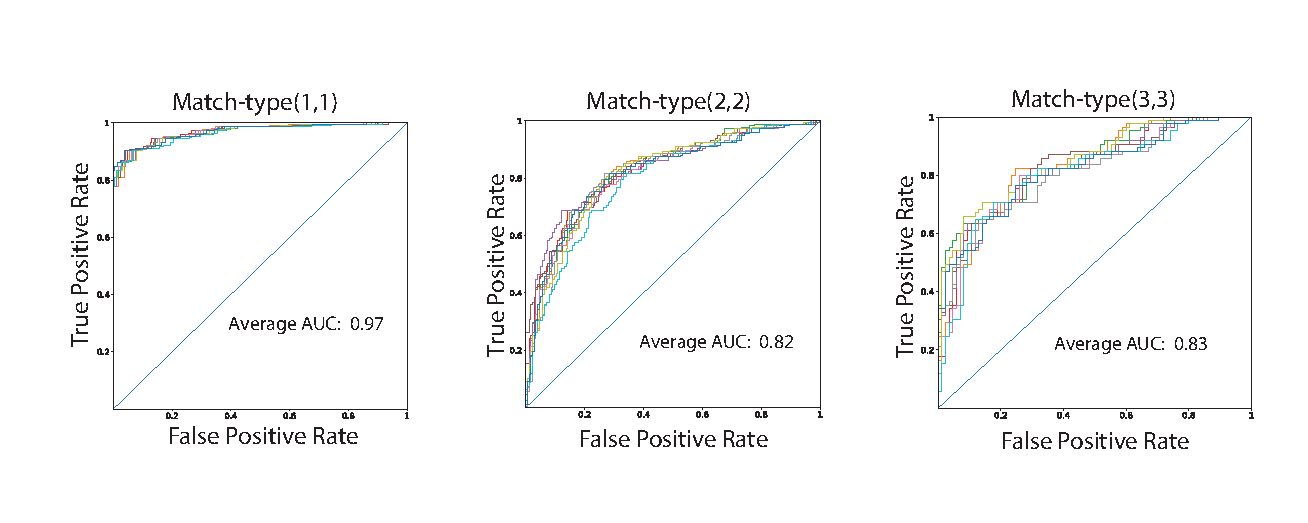
\includegraphics[scale=0.45]{Discrimination2-03.eps}
	\caption{\small{For each match-type, the testing were run on 10 independent testing set. The average AUC were calculated.}}
\end{figure}
\end{frame}

\begin{frame}
\frametitle{Testing the model}
\begin{figure}[H]
	\centering
	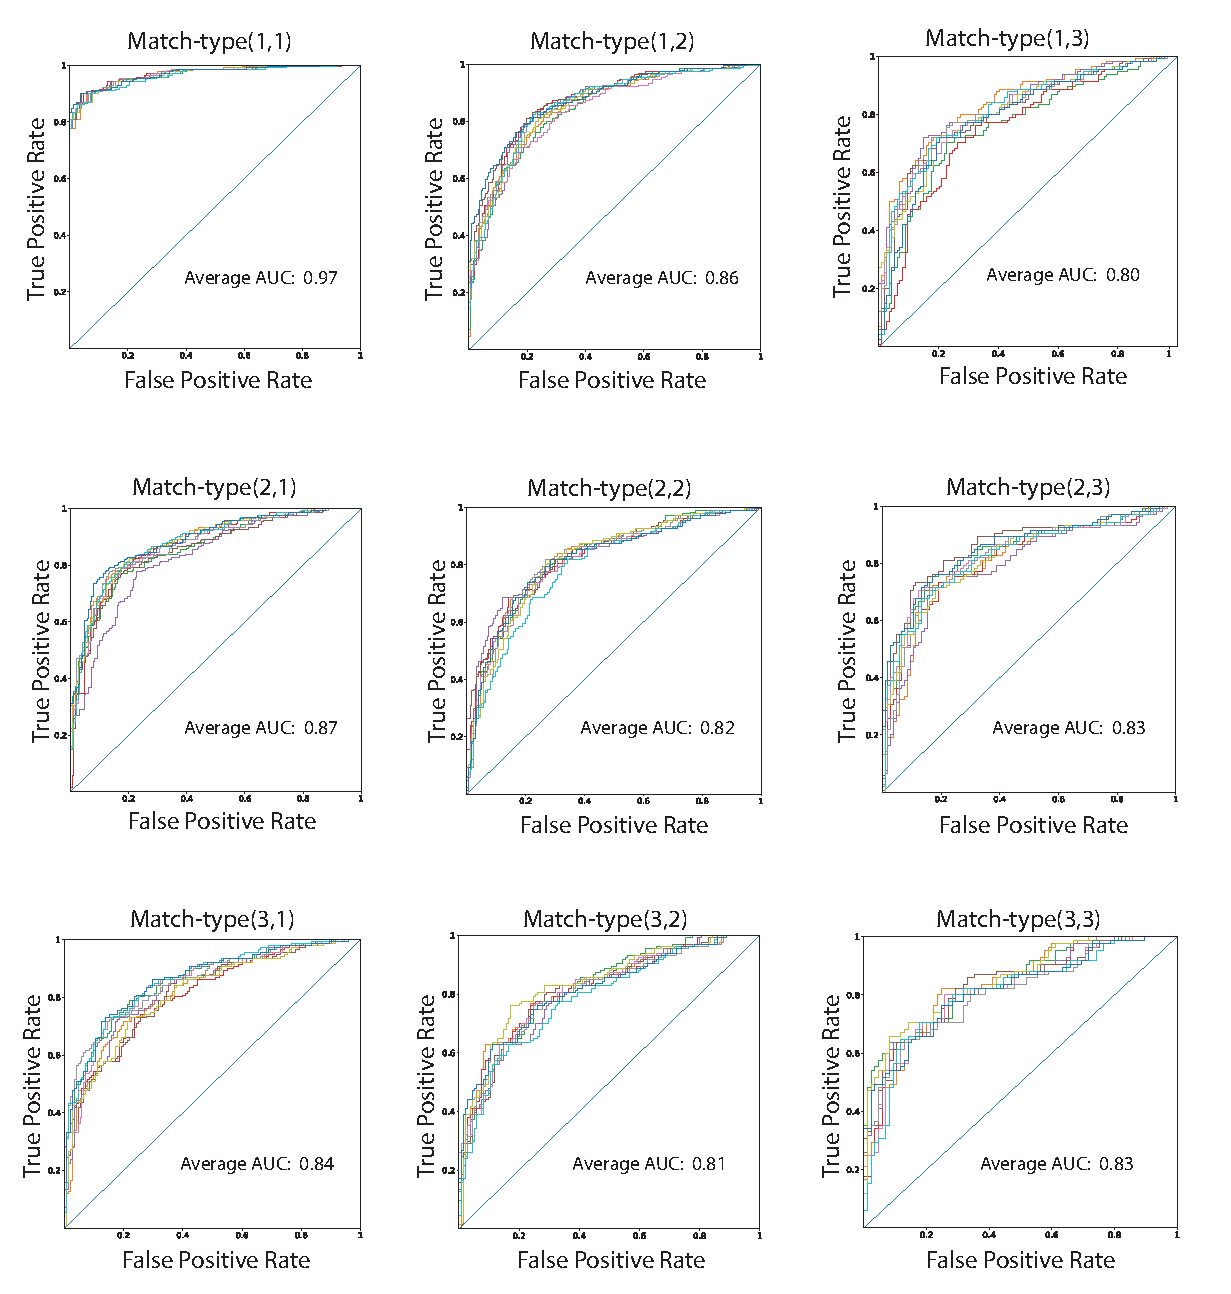
\includegraphics[scale=0.35]{PositiveNegativeDiscrimination.eps}
\end{figure}
\end{frame}


\section{ Applications of RBFN }
\subsection{Antibody aa and antigen aa are different}

\begin{frame}
\frametitle{Antibody aa and antigen aa are different}
Suppose (AbSeq, AgSeq) is of match-type(m,n). If there is no difference between AbSeq and AgSeq, then our model will not be able to tell the difference between (AgSeq, AbSeq) and a positive core of match-type(n,m).\vspace{0.5cm}

To prove the above statement, the testing set for each match-type was constructed as follows.
\begin{align*}
	\text{TR}_{(n, m)} &= \{(AgSeq, AbSeq):(AbSeq, AgSeq)\in \text{T}_{(m, n)}\}\\
	\text{T} &=\text{TR}_{(n, m)} \cup \text{T}_{(n, m)}
\end{align*}
Here T is the testing set of match-type(n,m).
\end{frame}

%\begin{frame}
%\frametitle{Antibody aa and antigen aa are different}
%\begin{figure}[H]
%	\centering
%	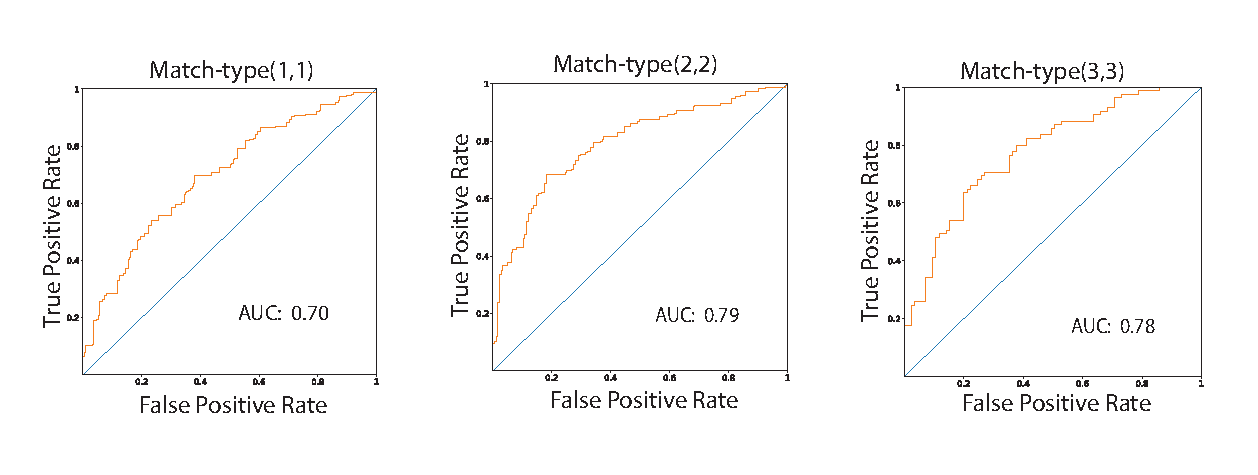
\includegraphics[scale=0.45]{Reverse1-03.eps}
%\end{figure}
%\end{frame}

\begin{frame}
\frametitle{Antibody aa and antigen aa are different}
\begin{figure}[H]
	\centering
	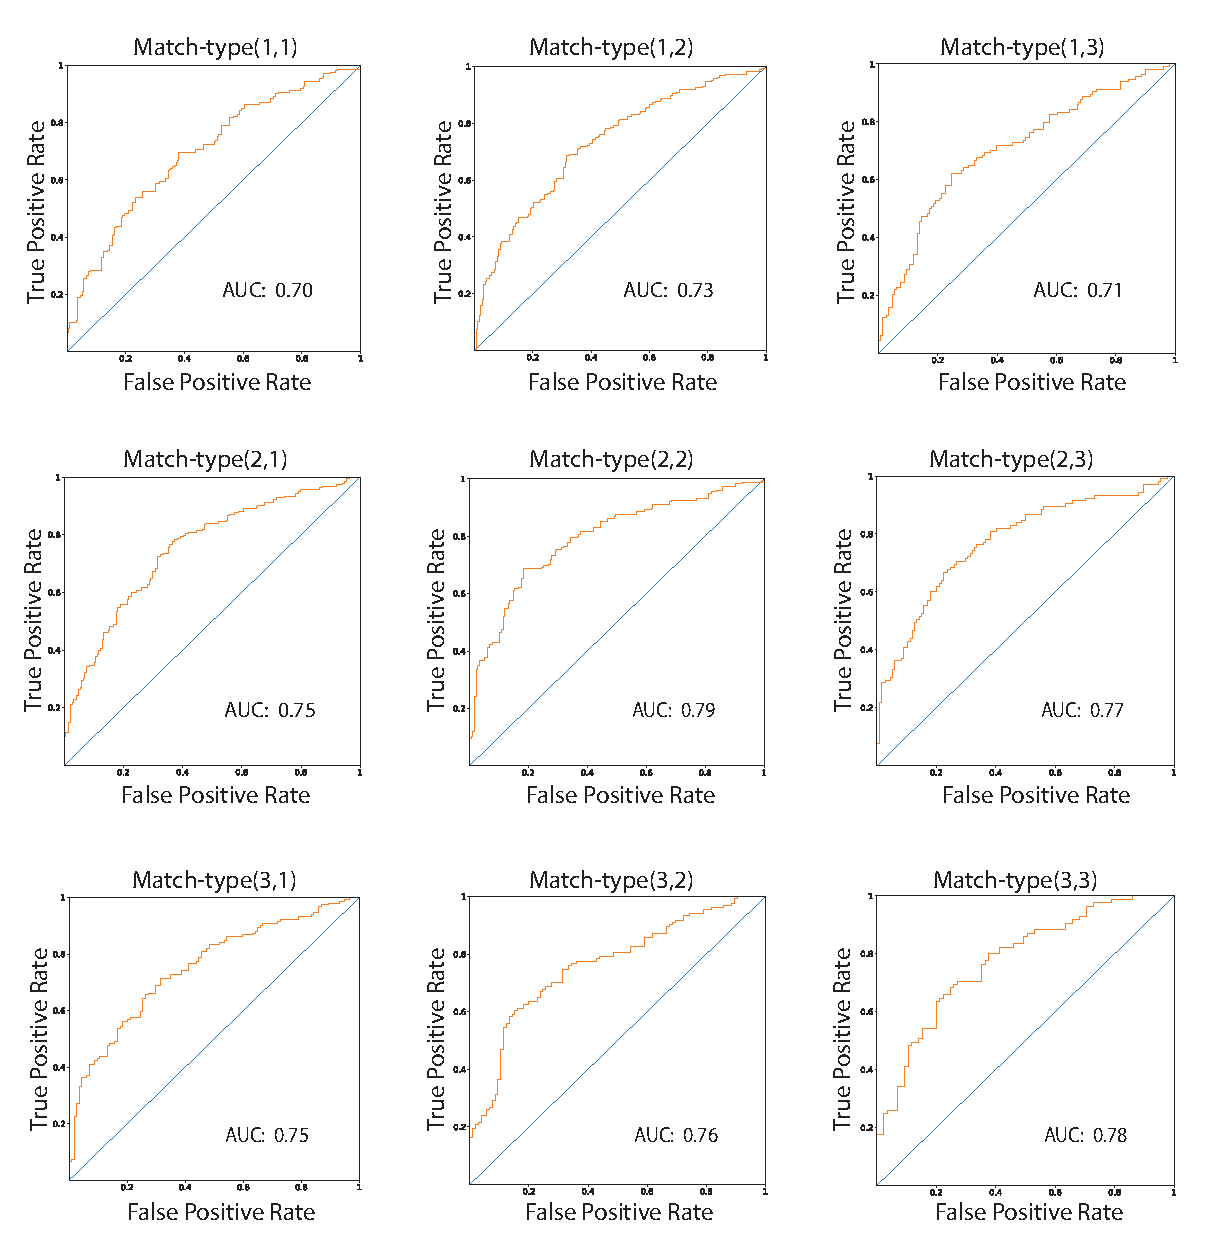
\includegraphics[scale=0.35]{Reverse.eps}
\end{figure}
\end{frame}
\subsection{RBFN can predict the affinity}
\begin{frame}
\frametitle{Basic assumptions}
\textbf{Assumption:} if a mutation changes the interacting sequences towards the direction of positive cores, then it increases the affinity.
\vspace{1cm}

\textbf{We uses the RBFN on match-type(1,1) to make predictions}
\end{frame}

\begin{frame}
\frametitle{Predictable Pairs}
\textbf{Step 1: Find the contacting pairs for each mutation.}
\begin{figure}
	\centering
	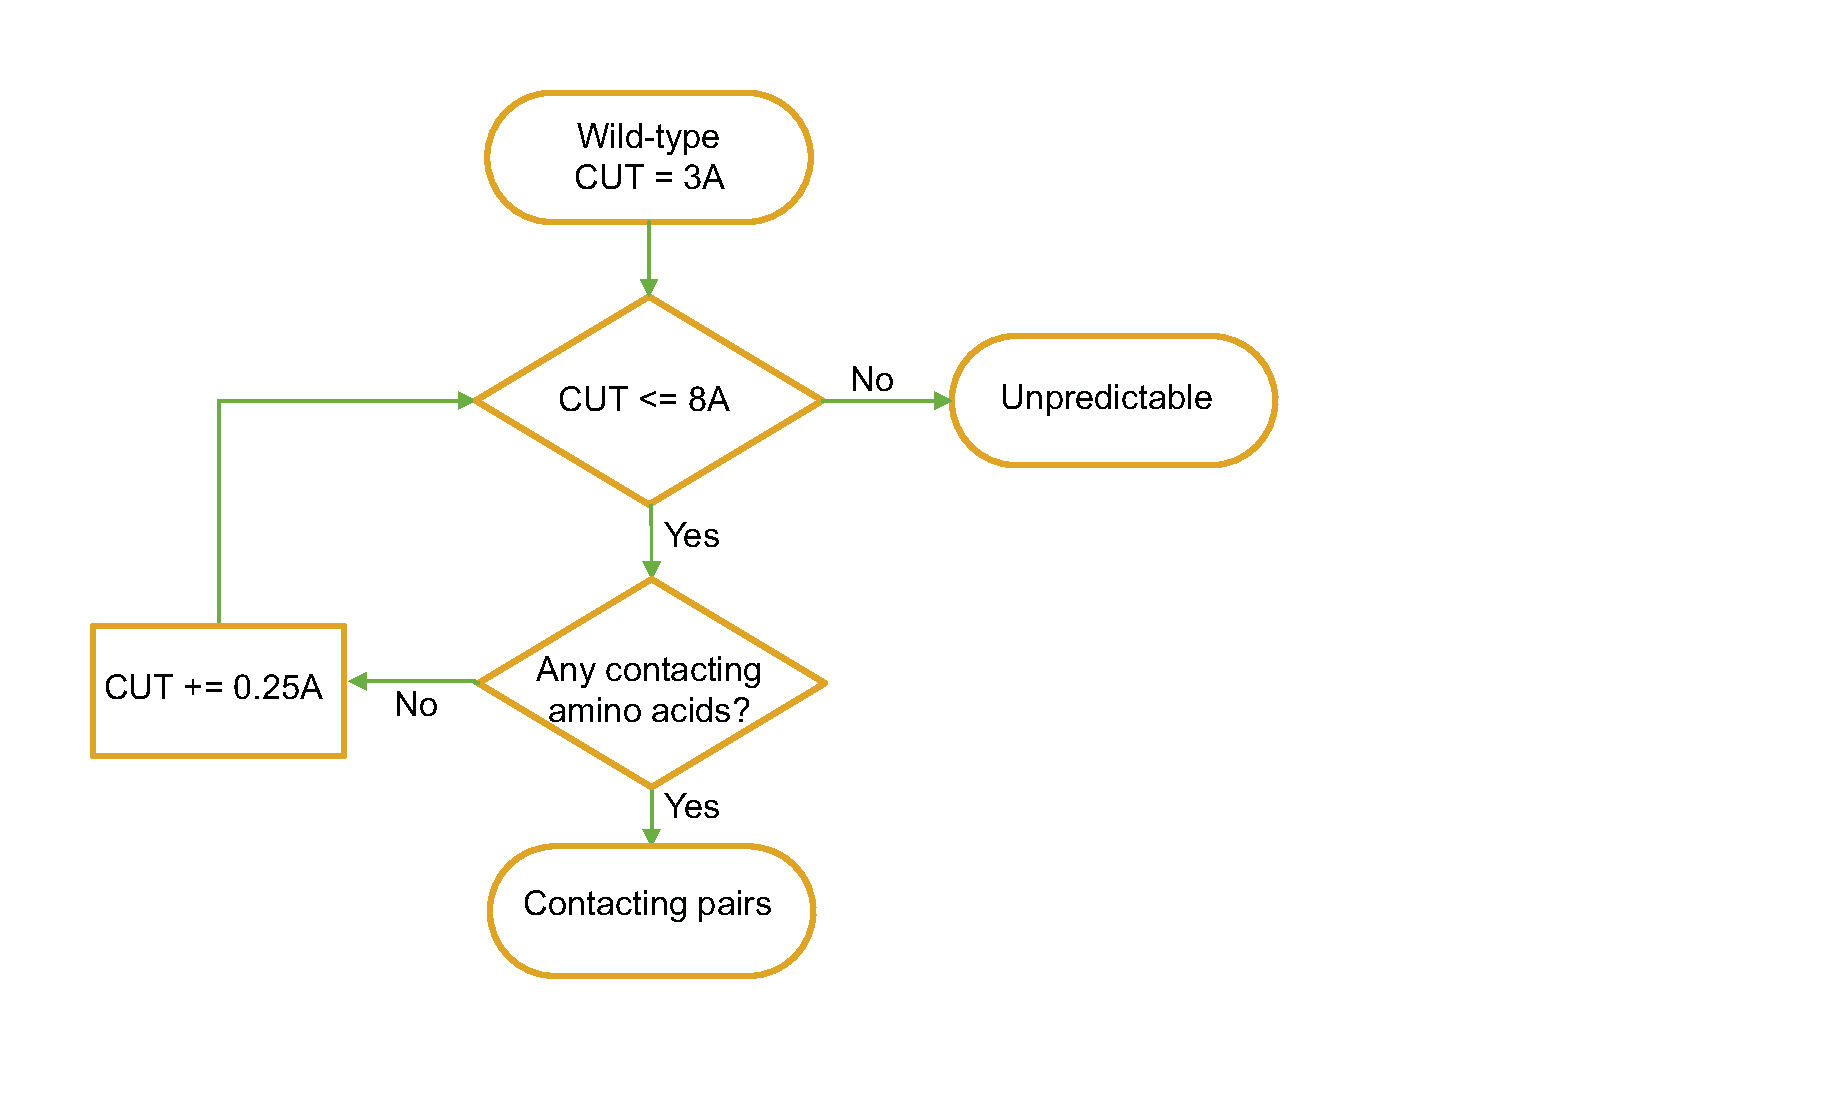
\includegraphics[scale=0.3]{ContactingPairs.eps}
\end{figure}
\end{frame}

\begin{frame}
\frametitle{Predictable Pairs}
\textbf{Step 2: Generate all predictable pairs}
\begin{figure}
	\centering
	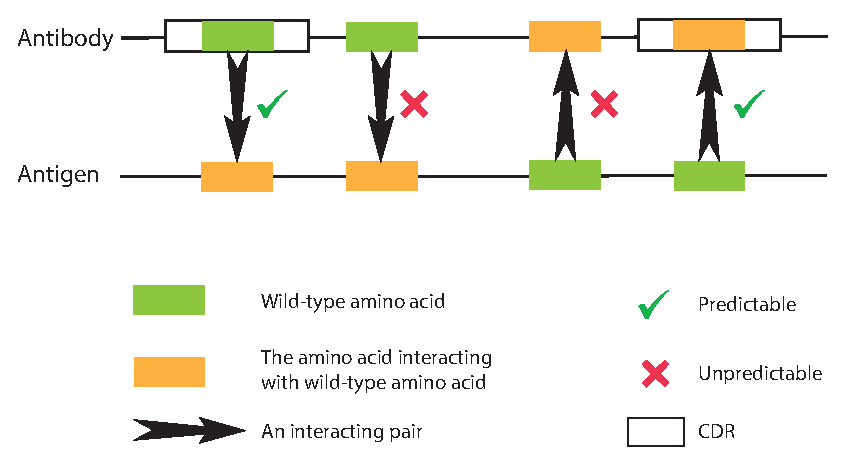
\includegraphics[scale=0.3]{Predictable.eps}
\end{figure}
\textbf{Step 3: For each mutation, pick the one with the largest contact number from the all the predictable pairs.}
\end{frame}

\begin{frame}
\frametitle{Make prediction}
Suppose there are two mutations, Mut1, Mut2, in a antibody-antigen complex. (Mut1, Ag1) and (Mut2, Ag2) are two predicable pairs. (Wt1, Ag1) and (Wt2, Ag2) are corresponding wild-type pairs. Calculate the change of the returned values by our RBFN model:
$$\Delta = \frac{1}{2}\sum\limits_{i=1,2} \left(RBFN(Muti, Agi)-RBFN(Wti, Agi)\right)$$
If $\Delta > 0$, the affinity increases. If $\Delta <0$ the affinity decreases.

\end{frame}

\begin{frame}
\frametitle{Results}
\begin{figure}
	\centering
	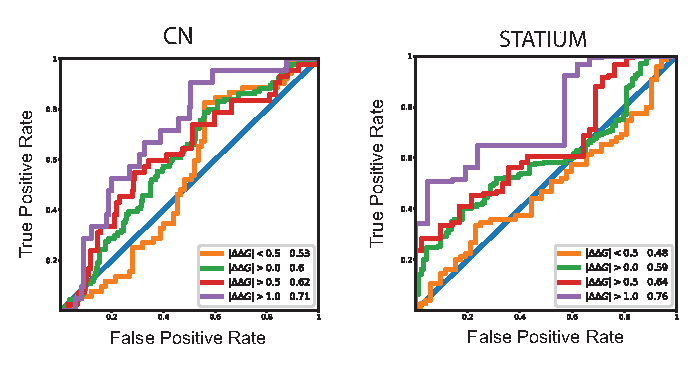
\includegraphics[scale=0.8]{CNStatium.eps}
\end{figure}
\end{frame}

\begin{frame}
\frametitle{Results}
\begin{table}[H]
\centering
\resizebox{\textwidth}{2cm}{
\begin{tabular}{ccccc}
\hline\hline
            & $\Delta\Delta G < 0.5$  & $\Delta\Delta G >0$ & $\Delta\Delta G > 0.5$ & $\Delta\Delta G > 1$  \\
\hline
CN&(0.43, 0.63)& (0.54, 0.66)&(0.53, 0.71)&(0.60, 0.80)
\\
bASA&(0.44, 0.64)& (0.58, 0.69)&(0.57, 0.74)&(0.54, 0.80)
\\
dfire&(0.45, 0.67)& (0.62, 0.73)&(0.63, 0.79)&(0.67, 0.84)
\\
dDfire&(0.50, 0.71)& (0.57, 0.68)&(0.54, 0.70)&(0.57, 0.78)
\\
Rosetta&(0.37, 0.68)& (0.57, 0.68)&(0.59, 0.76)&(0.67, 0.87)
\\
STATIUM&(0.42, 0.63)& (0.57, 0.68)&(0.58, 0.75)&(0.68, 0.87)
\\
D Studio&(0.48, 0.69)& (0.67, 0.77)&(0.70, 0.83)&(0.77, 0.92)
\\
FoldX&(0.51, 0.71)& (0.69, 0.8)&(0.79, 0.91)&(0.86, 0.98)
\\
\hline
\end{tabular}
}
\caption{ 95\% confidence intervals constructed by Bootstrap. The iteration number is 10,000. D Studio is short for Discovery Studio.}
\label{Bootstrap}
\end{table}
\end{frame}
%\begin{frame}
%\frametitle{blocs}
%
%\begin{block}{title of the bloc}
%bloc text
%\end{block}
%
%\begin{exampleblock}{title of the bloc}
%bloc text
%\end{exampleblock}
%
%
%\begin{alertblock}{title of the bloc}
%bloc text
%\end{alertblock}
%\end{frame}

\end{document}

